\documentclass[11pt,a4paper]{article}
\usepackage[T1]{fontenc}
\usepackage[utf8]{inputenc}
\usepackage{lmodern}
\usepackage{amsmath,amssymb,amsthm,mathtools}
\usepackage{microtype}
\usepackage[a4paper,margin=27mm,headheight=14pt,headsep=8mm]{geometry}
\usepackage{booktabs,tabularx,array}
\usepackage{tikz}
\usetikzlibrary{arrows.meta,positioning,calc}
\usepackage{enumitem}
\usepackage{fancyhdr}
\usepackage{xcolor}
\usepackage{hyperref}
\usepackage{url}
\definecolor{deep}{HTML}{16243D}
\definecolor{accent}{HTML}{346BA1}
\definecolor{soft}{HTML}{687A91}
\definecolor{cream}{HTML}{F2F5F9}
\hypersetup{colorlinks=true,linkcolor=deep,citecolor=accent,urlcolor=accent,pdftitle={Mod-two cohomology of a central quotient of the Weyl group of type F4},pdfauthor={Xorch}}
\urlstyle{same}
\pagestyle{fancy}
\fancyhf{}
\fancyhead[L]{\sffamily\footnotesize\textcolor{soft}{CONCORDANTE LAB \quad/\quad MATHEMATICAL RESEARCH}}
\fancyhead[R]{\sffamily\footnotesize\textcolor{soft}{PREPRINT 0.1-public}}
\fancyfoot[C]{\sffamily\footnotesize\textcolor{soft}{\thepage}}
\renewcommand{\headrulewidth}{0.25pt}
\renewcommand{\headrule}{\hbox to\headwidth{\color{soft!50}\leaders\hrule height \headrulewidth\hfill}}
\setlength{\parindent}{0pt}
\setlength{\parskip}{0.48em}
\setlist[itemize]{topsep=3pt,itemsep=2pt,leftmargin=17pt}
\setlist[enumerate]{topsep=3pt,itemsep=2pt,leftmargin=20pt}
\newtheorem{theorem}{Theorem}[section]
\newtheorem{lemma}[theorem]{Lemma}
\newtheorem{proposition}[theorem]{Proposition}
\newtheorem{corollary}[theorem]{Corollary}
\theoremstyle{remark}\newtheorem{remark}[theorem]{Remark}
\newcommand{\F}{\mathbb F}
\newcommand{\Z}{\mathbb Z}
\newcommand{\GG}{\mathcal G}
\newcommand{\CP}{\mathcal P}
\newcommand{\HH}{\mathrm H}
\newcommand{\Sym}{\operatorname{Sym}}
\newcommand{\res}{\operatorname{res}}
\newcommand{\cor}{\operatorname{cor}}
\newcommand{\Span}{\operatorname{span}}
\newcommand{\Ind}{\operatorname{Ind}}
\newcommand{\depth}{\operatorname{depth}}
\newcommand{\Hilb}{\operatorname{Hilb}}
\newcommand{\mm}{\,\mathrm{mod}\,}
\newcommand{\w}{\mathit w}
\newcommand{\unit}{\mathds{1}}
\setcounter{tocdepth}{2}
\begin{document}
\thispagestyle{empty}
\vspace*{-6mm}
\begin{minipage}[t]{0.72\linewidth}
{\sffamily\fontsize{10}{12}\selectfont\bfseries\textcolor{accent}{CONCORDANTE LAB \quad / \quad RESEARCH PREPRINT}}\\[2.5mm]
{\color{soft}\rule{\linewidth}{0.7pt}}
\end{minipage}\hfill
\begin{minipage}[t]{0.22\linewidth}
\raggedleft\sffamily\footnotesize\textcolor{soft}{21 OCT 2026\\VERSION 0.1-public}
\end{minipage}
\vspace{7mm}

{\color{deep}\sffamily\bfseries\fontsize{23}{28}\selectfont
The mod-two cohomology ring\\[1mm]
of a central quotient of\\[1mm]
the Weyl group of type \(F_4\)\par}
\vspace{4mm}
{\sffamily\large\textcolor{soft}{Invariant theory, Sylow transfer, and an explicit finite presentation}\par}
\vspace{8mm}
\begin{minipage}[t]{0.62\linewidth}
{\large\bfseries Xorch}\\[1.4mm]
{\sffamily\textcolor{soft}{Concordante Lab \quad | \quad Independent research}}\\[2mm]
\textcolor{soft}{\small \copyright\ 2026 Xorch --- Concordante Lab.}
\end{minipage}\hfill
\begin{minipage}[t]{0.34\linewidth}
\centering
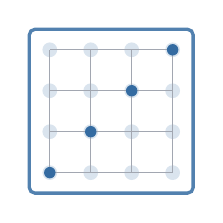
\begin{tikzpicture}[scale=0.52,baseline=5mm]
\foreach \x in {0,1,2,3}{\foreach \y in {0,1,2,3}{
  \fill[accent!18] (\x,\y) circle(0.18);
}}
\foreach \x in {0,1,2,3}{\draw[deep!40,line width=0.45pt] (\x,0)--(\x,3);}
\foreach \y in {0,1,2,3}{\draw[deep!40,line width=0.45pt] (0,\y)--(3,\y);}
\foreach \x/\y in {0/0,1/1,2/2,3/3}{\fill[accent] (\x,\y) circle(.14);}
\draw[accent!85,line width=1.2pt,rounded corners=2pt] (-0.5,-0.5) rectangle(3.5,3.5);
\end{tikzpicture}
\end{minipage}
\vspace{6mm}

\noindent\colorbox{cream}{\parbox{\dimexpr\linewidth-2\fboxsep}{\small\sffamily
\textbf{Research manuscript for independent mathematical verification.} This edition includes the complete written argument, explicit algebraic input and bounded checks. The ring-isomorphism theorem is conditional on the authenticated global-class and ideal certificates specified in Section~9; assembling and independently replaying that full bundle is the next verification step.}}
\vspace{6mm}
\section*{Abstract}
Let \(G=W(F_4)/\{\pm I\}\) be the order-576 central quotient of the Weyl group of type \(F_4\), identified with \(V\rtimes(S_3\times S_3)\), where \(V\cong(C_2)^4\) carries the tensor product of two natural two-dimensional \(\F_2\)-representations. We present a reproducible computation of \(\HH^*(G;\F_2)\) with eight explicit homogeneous generators and nine homogeneous defining relations. The proof combines a Nakaoka collapse for the regular wreath-product Sylow subgroup, odd-index restriction, an invariant-fiber calculation, Shapiro's lemma, and certified Gr\"obner arithmetic. In particular we derive an all-degree rational Hilbert--Poincar\'e series and recover \(\dim\HH^{19}(G;\F_2)=141\). The manuscript specifies the finite certificates on which its computational steps depend and separates the mod-two ring from unresolved integral and secondary operations. It is offered for independent verification, with historical-priority assessment reserved for a dedicated literature review.

\textbf{Keywords:} finite group cohomology; Weyl group; \(F_4\); invariant theory; Sylow subgroup; Lyndon--Hochschild--Serre spectral sequence; Gr\"obner basis; computer-assisted proof.

\textbf{Mathematics Subject Classification (2020):} 20J06, 55T10, 13P10, 20C20.
\vspace{2mm}
\hrule
\vspace{3mm}
{\small\textbf{Resumen.} Se presenta una descripci\'on verificable de la cohomolog\'ia m\'odulo dos del cociente central de \(W(F_4)\): ocho generadores, nueve relaciones y una serie de Poincar\'e exacta en todos los grados. Se distinguen los argumentos te\'oricos cl\'asicos, los certificados computacionales y las cuestiones de cohomolog\'ia integral que siguen abiertas.}
\newpage
\tableofcontents
\vspace{3mm}\hrule\vspace{4mm}

\section{Introduction and statement of the result}
Cohomology rings of finite groups are natural meeting points of modular representation theory, group extensions, homological algebra, and computational commutative algebra. The present calculation concerns the finite quotient
\begin{equation}\label{eq:group}
G=W(F_4)/\{\pm I\}\cong V\rtimes Q,\qquad
V=(C_2)^4,\quad Q=S_3\times S_3,
\end{equation}
where the \(Q\)-action on \(V\) is the tensor product of its two standard \(\F_2^2\)-representations. Thus \(|G|=16\cdot36=576\). The abstract group also occurs as \texttt{SmallGroup(576,8654)} in GAP-compatible catalogs \cite{gapchar}.

Put \(k=\F_2\). Denote by \(x,y,\alpha,\gamma,w_4,w_5,w_6,\Theta\) homogeneous classes of respective degrees
\[
(1,1,2,3,4,5,6,6).
\]
Their construction uses authentic group characters, a central-extension class, and polynomial characteristic-class restrictions; the polynomial inputs are specified in the machine-readable accompanying data. In particular, \(\gamma=\mathrm{Sq}^1(\alpha)\).

\begin{theorem}[Explicit graded ring, conditional theorem]\label{thm:ring}
Let
\[
A=k[x,y,\alpha,\gamma,w_4,w_5,w_6,\Theta]
\]
with the indicated weights, and let \(J\subset A\) be generated by the nine homogeneous relations \(R_3,R_{4a},R_{4b},R_{6a},R_{6b},R_{7a},R_{7b},R_{10},R_{12}\) in \S\ref{sec:relations}. Subject to the authenticated computational inputs specified in \S\ref{sec:certificates}, the natural evaluation homomorphism induces an isomorphism of \emph{graded algebras in every degree},
\begin{equation}\label{eq:main}
A/J\ \xrightarrow{\ \sim\ }\ \HH^*(G;k).
\end{equation}
The Hilbert--Poincar\'e series is
\begin{equation}\label{eq:hilbert}
\boxed{\quad
P_G(t)=\sum_{n\ge0}\dim_k\HH^n(G;k)t^n
=\frac{1+2t^2-t^3+t^4-t^8-t^9}
{(1-t)^2(1-t^3)(1+t^2)(1-t^6)}.\quad}
\end{equation}
\end{theorem}

The proof uses all-degree structural arguments. Its infinite-degree steps use classical theorems of Nakaoka, restriction/transfer, and Shapiro \cite{nakaoka,brown,cts}. The computational components are two polynomial identities on the normal elementary-abelian fiber, authentic evaluations of nine global relations, and an exact Hilbert-series computation of their quotient.

\paragraph{Contribution and scope.}
The result presents \(\HH^*(G;k)\) as a graded algebra, with explicit generators, relations and a rational Hilbert series. The all-degree integral ring, higher Bocksteins and Massey products form separate research questions. The Steenrod formulas are documented in a separate companion note. Historical-priority assessment and external peer review remain subsequent editorial steps.

\section{The structural proof architecture}
\begin{center}
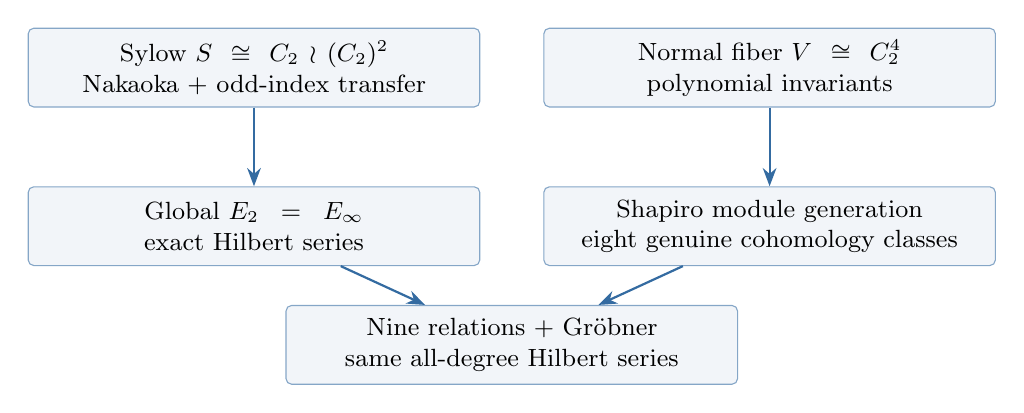
\begin{tikzpicture}[node distance=10mm and 8mm,>=Stealth,
  block/.style={draw=accent!60,fill=cream,rounded corners=2pt,align=center,
               text width=55mm,minimum height=10mm,font=\small}]
\node[block] (s) {Sylow \(S\cong C_2\wr (C_2)^2\)\\Nakaoka + odd-index transfer};
\node[block,right=of s] (f) {Normal fiber \(V\cong C_2^4\)\\polynomial invariants};
\node[block,below=of s] (h) {Global \(E_2=E_\infty\)\\exact Hilbert series};
\node[block,below=of f] (g) {Shapiro module generation\\eight genuine cohomology classes};
\node[block,below=of $(h)!0.5!(g)$] (r) {Nine relations + Gr\"obner\\same all-degree Hilbert series};
\draw[->,accent,thick] (s)--(h);
\draw[->,accent,thick] (f)--(g);
\draw[->,accent,thick] (h)--(r);
\draw[->,accent,thick] (g)--(r);
\end{tikzpicture}
\end{center}
The two independent axes are \emph{dimension} (spectral sequence and Hilbert series) and \emph{multiplication} (genuine global classes and invariant-fiber generation). Equality of Hilbert series alone would not establish \eqref{eq:main}; the multiplicative filtered-generation argument is essential.

\section{Global collapse of the LHS spectral sequence}\label{sec:collapse}
Consider
\begin{equation}\label{eq:lhs}
E_2^{p,q}=\HH^p\!\left(Q;\HH^q(V;k)\right)
=\HH^p\!\left(Q;\Sym^q(V^*)\right)
\ \Longrightarrow\ \HH^{p+q}(G;k).
\end{equation}
Let \(P=C_2\times C_2\) be a Sylow 2-subgroup of \(Q\), and \(S=V\rtimes P\subset G\); then \([G:S]=9\).

\begin{lemma}\label{lem:wreath}
As a \(k[P]\)-module, \(V\) is the regular permutation module \(k[P]\). Consequently \(S\cong C_2\wr P\), the wreath product with four-element regular \(P\)-set.
\end{lemma}
\begin{proof}
Each transposition in \(S_3\cong\mathrm{GL}_2(k)\) is a nontrivial unipotent involution. After choosing a suitable basis, it swaps two basis vectors. Taking tensor products, the two order-two generators of \(P\) act on the four tensor basis vectors by flipping the first and second indices respectively. The resulting \(P\)-set is regular. The underlying additive group of \(V\) is therefore the fourfold \(C_2\)-base of the regular wreath product.
\end{proof}

\begin{proposition}[All-degree additive collapse]\label{prop:collapse}
Every differential \(d_r\), \(r\ge2\), of the spectral sequence \eqref{eq:lhs} vanishes. Hence its \(E_2\) and \(E_\infty\) pages coincide as bigraded vector spaces.
\end{proposition}
\begin{proof}
The Nakaoka wreath-product theorem gives the collapse at \(E_2\) for the extension \(V\to S\to P\) with coefficients in \(k\) \cite{nakaoka,cts}. For every \(k[Q]\)-module \(M\) and every \(p\), restriction \(\HH^p(Q;M)\to\HH^p(P;M)\) is injective, since restriction followed by corestriction acts on the source by \([Q:P]=9=1\) in \(k\). In particular, the map of LHS spectral sequences induced by \(S\subset G\) is injective on \(E_2\). If a differential for \(G\) were first nonzero on some page \(r\), the earlier pages would still have the same \(E_2\) terms, so naturality and injectivity in the target would contradict the corresponding zero differential for \(S\). Thus all differentials vanish. The assertion is \emph{additive}: a multiplicative identification with \(E_2\) does not follow from collapse alone.
\end{proof}

\section{An all-degree rational Poincar\'e series}\label{sec:series}
Write \(K=C_3\times C_3\trianglelefteq Q\). The quotient \(Q/K\) is \(P=C_2^2\), and the normal subgroup \(K\) has order invertible in \(k\). Therefore
\[\HH^p(Q;\Sym^q V^*)\cong\HH^p(P;(\Sym^qV^*)^K).\]
Extending scalars to \(\F_4\) diagonalizes \(K\) without changing dimensions. Let \(a,b,c,d\) denote variables with the four \(K\)-characters \((1,1),(1,-1),(-1,1),(-1,-1)\). A monomial \(a^A b^B c^C d^D\) is \(K\)-invariant if and only if
\begin{equation}\label{eq:monomial-condition}
A\equiv D\pmod3,\qquad B\equiv C\pmod3.
\end{equation}
The residual \(P\) acts by the commuting swaps \((a,b,c,d)\mapsto(c,d,a,b)\) and \((a,b,c,d)\mapsto(b,a,d,c)\). Let \(u_q,v_q,w_q\) count the orbits of lengths \(1,2,4\), respectively, among the invariant monomials of degree \(q\).

\begin{lemma}[Orbit contributions]\label{lem:shapiro-dims}
For \(p\ge0\),
\[
\dim_k E_2^{p,q}=\begin{cases}
 u_q+v_q+w_q,&p=0,\\
 (p+1)u_q+v_q,&p>0.
\end{cases}
\]
\end{lemma}
\begin{proof}
The orbit permutation module of length \(j=1,2,4\) is induced from the trivial module of a stabilizer of respective order \(4,2,1\). By Shapiro, its cohomology is that of \(C_2^2,C_2,1\): dimensions \(p+1,1,0\) in positive degree, and dimension one in degree zero. Descend from \(\F_4\) to \(k\).
\end{proof}

The generating function for pairs of nonnegative exponents congruent modulo three is
\[F(t)=\frac{1+t^2+t^4}{(1-t^3)^2}.\]
Denote the total invariant-monomial series by \(M(t)=F(t)^2\), and set \(C(t)=(1-t^4)^{-1}\). Burnside counting over the \emph{ordinary integers} gives
\begin{align*}
A(t)&:=\sum_{q\ge0}(u_q+v_q+w_q)t^q
=\frac{M(t)+2F(t^2)+(1-t^2)^{-2}}4,\\
B(t)&:=\sum_{q\ge0}v_qt^q
=\frac{2F(t^2)+(1-t^2)^{-2}-3C(t)}2,\\
\sum_{q\ge0}u_qt^q&=C(t).
\end{align*}
The fractions here count integral orbit averages; they are not operations of dividing by two or four inside \(\F_2\). By Lemma \ref{lem:shapiro-dims} and Proposition \ref{prop:collapse},
\[
P_G(t)=A(t)+\frac{t}{1-t}B(t)+\left(\frac1{(1-t)^2}-1\right)C(t).
\]
Integer rational-function simplification yields exactly \eqref{eq:hilbert}.

\begin{center}
\small
\begin{tabular}{@{}r|rrrrrrrrrrr@{}}
\toprule
\(n\) &0&1&2&3&4&5&6&7&8&9&10\\ \midrule
\(b_n\)&1&2&4&6&8&12&17&21&27&33&39\\
\midrule
\(n\) &11&12&13&14&15&16&17&18&19&20&\\ \midrule
\(b_n\)&48&57&65&77&88&98&113&128&141&159&\\
\bottomrule
\end{tabular}
\end{center}
These are the dimensions of \(\HH^n(G;k)\), not merely spectral-sequence upper bounds. In fact, the series has an all-degree period-12 quasipolynomial formula: for \(n=12m+r\), \(0\le r<12\),
\begin{equation}\label{eq:quasi}
 b_{12m+r}=a_r+c_rm+(122+4r)\binom m2+48\binom m3,
\end{equation}
where
\begin{align*}
(a_0,\dots,a_{11})&=(1,2,4,6,8,12,17,21,27,33,39,48),\\
(c_0,\dots,c_{11})&=(56,63,73,82,90,101,111,120,132,143,153,166).
\end{align*}
The all-degree identity, rather than finite interpolation, follows because the rational denominator divides \((1-t^{12})^4\); the initial polynomial coefficients determine the four nonzero finite-difference layers.

\section{The ring of normal-fiber invariants}\label{sec:fiber}
The crucial multiplicative input is a presentation of the invariant ring \(k[V^*]^Q\). Consider the genuine restricted classes \(\alpha,\gamma,w_4,w_5,w_6,\Theta\). Their full polynomial supports in four variables \(t_0,t_1,t_2,t_3\) are provided in \texttt{f4\_algebra\_data.json}. Write
\[C=k[\alpha,\gamma,w_4,w_6]\]
and define
\begin{equation}\label{eq:Bfiber}
B=\frac{k[\alpha,\gamma,w_4,w_5,w_6,\Theta]}
{(R_{10}^{V},R_{12}^{V})},
\end{equation}
where
\begin{align}
R_{10}^{V}={}&w_5^2+\alpha\gamma w_5+\gamma^2w_4+\alpha^2w_6+\alpha^5,\label{eq:fiber10}\\
R_{12}^{V}={}&\Theta^2+(w_6+\gamma^2+\alpha^3)\Theta\notag\\
&+\gamma w_4w_5+\alpha\gamma^2w_4
+\alpha^2w_4^2+\alpha^3\gamma^2.\label{eq:fiber12}
\end{align}
The data check these are literal zero polynomial identities after substitution of the recorded four-variable supports.

\begin{proposition}[Explicit invariant fiber]\label{prop:fiber}
The natural map \(B\to k[V^*]^Q\) induced by restriction is an isomorphism. The \(C\)-module \(B\) is free of rank four on \(1,w_5,\Theta,w_5\Theta\).
\end{proposition}
\begin{proof}
The two equations are monic in \(w_5^2\) and, successively, \(\Theta^2\), which supplies the stated free basis. In particular,
\begin{equation}\label{eq:fiber-hilbert}
\Hilb_B(t)=\frac{1+t^5+t^6+t^{11}}
{(1-t^2)(1-t^3)(1-t^4)(1-t^6)}.
\end{equation}
For completeness we describe the injectivity certificate. Over \(\mathrm{Frac}(C)\), abbreviate \(a=\alpha,g=\gamma,u=w_4,w=w_6,v=w_5,h=\Theta\), and set
\begin{align*}
A_0&=g^2u+a^2w+a^5,&B_0&=w+g^2+a^3,\\
C_0&=gu,&D_0&=ag^2u+a^2u^2+a^3g^2.
\end{align*}
The two equations become \(v^2+agv+A_0=0\) and \(h^2+B_0h+C_0v+D_0=0\). Eliminating \(v\) gives the monic quartic
\[
\mathcal F(T)=(T^2+B_0T+D_0)^2+agC_0(T^2+B_0T+D_0)+A_0C_0^2.
\]
At \(a=g=u=w=1\), this specializes to \(T^4+T+1\), irreducible over \(\F_2\). Monicity and Gauss's lemma give irreducibility over \(\mathrm{Frac}(C)\); freeness then shows \(B\) is a domain.

The four explicit fiber polynomials for \(\alpha,\gamma,w_4,w_6\), ordered by the weighted monomial order with weights \((1,3,3,4)\), have leading exponent rows
\[
\begin{pmatrix}0&1&1&0\\1&0&0&2\\0&0&0&4\\0&2&0&4\end{pmatrix},
\qquad \det=-8\ne0\ \text{in }\Z.
\]
Their leading monomials are therefore multiplicatively independent, proving algebraic independence of those four elements. It is \emph{nonzero integer determinant}, not nonzero determinant modulo two, that is used. The induced prime kernel \(B\to k[V^*]^Q\) must be zero: a nonzero prime ideal of the four-dimensional domain \(B\) would decrease transcendence degree, whereas the image contains four algebraically independent invariants.

Finally, the Burnside invariant-ring series \(A(t)\) from \S\ref{sec:series} equals \eqref{eq:fiber-hilbert} as a rational function. Injectivity and equality of each graded dimension give surjectivity.
\end{proof}

\section{From Shapiro to global generators}\label{sec:generation}
A subtle point is that collapse of \eqref{eq:lhs} as a \emph{vector-space} spectral sequence does not automatically identify cup products. We avoid assuming a multiplicative splitting.

\begin{lemma}[Module generation on the \(E_2\)-page]\label{lem:shapiro}
The bigraded \(E_2\)-algebra is generated by its two edge algebras
\[
E_2^{0,*}=k[V^*]^Q\quad\text{and}\quad E_2^{*,0}=\HH^*(Q;k)=k[x,y].
\]
\end{lemma}
\begin{proof}
Over \(\F_4\), \(K\)-invariant monomials form a permutation basis for \(P\). For any orbit \(\Omega\), let \(H\le P\) be the stabilizer of a point. Shapiro identifies the contribution to \(E_2\) with \(\HH^*(H;\F_4)\), and the invariant orbit sum maps to its unit. Multiplication by an inflated base class corresponds to \(\res_H^P:\HH^*(P;\F_4)\to\HH^*(H;\F_4)\). This map is surjective for \(H=P,C_2,1\). Hence every orbit summand is a module over the base ring generated in filtration degree zero. Direct sums and faithfully flat descent from \(\F_4\) to \(k\) establish the statement.
\end{proof}

\begin{lemma}[Finite filtered lifting]\label{lem:filtered}
Let \(R\) be a connected, nonnegatively graded algebra with a finite decreasing multiplicative filtration in each degree. If the initial symbols of homogeneous classes \(z_1,\dots,z_m\) generate \(\operatorname{gr}_F R\), then the \(z_i\) generate \(R\).
\end{lemma}
\begin{proof}
Given a homogeneous \(r\in F^pR\), choose a polynomial \(h(z_i)\) whose initial symbol agrees with that of \(r\). Subtracting raises the filtration index. Repeating terminates because the filtration is finite in the chosen total degree. The resulting sum of polynomials equals \(r\).
\end{proof}

\begin{proposition}\label{prop:surj}
The evaluation homomorphism \(A\to\HH^*(G;k)\) is surjective in every degree.
\end{proposition}
\begin{proof}
Proposition \ref{prop:fiber} identifies the six restricted global classes as generators of \(E_2^{0,*}\), and the group characters \(x,y\) generate \(E_2^{*,0}\). Lemma \ref{lem:shapiro} thus generates all of \(E_2\) from the eight initial symbols. Proposition \ref{prop:collapse} identifies \(E_\infty\) with \(E_2\) as associated-graded terms. Multiplicativity of the LHS filtration and Lemma \ref{lem:filtered} finish the argument.
\end{proof}

\section{Nine explicit relations and the computational closure}\label{sec:relations}
For auditability, here are \emph{all nine} homogeneous polynomials that define \(J\); coefficients are in \(\F_2\). The labels indicate their cohomological weights.
\begin{align}
R_3={}&y\alpha,\label{eq:r3}\\
R_{4a}={}&y\gamma,\\
R_{4b}={}&x\gamma+x^2\alpha,\\
R_{6a}={}&yw_5+xyw_4+xy^5+x^2y^4,\\
R_{6b}={}&xw_5+x^2w_4+x^2y^4+x^3y^3,\\
R_{7a}={}&y\Theta+x\Theta+x\alpha w_4+x^4\gamma,\label{eq:r7a}\\
R_{7b}={}&x\Theta+xw_6+x\alpha w_4+x\alpha^3
+xyw_5+xy^2w_4\notag\\
&+xy^6+x^2yw_4+x^3w_4+x^5y^2+x^6y+x^7,\label{eq:r7b}\\
R_{10}={}&w_5^2+\gamma^2w_4+\alpha\gamma w_5+\alpha^2w_6+\alpha^5\notag\\
&+xw_4w_5+x\gamma\Theta+x\gamma^3+xy^4w_5+x^2y^3w_5,\label{eq:r10}\\
R_{12}={}&\Theta^2+w_6\Theta+\gamma w_4w_5+\gamma^2\Theta
+\alpha\gamma^2w_4\notag\\
&+\alpha^2w_4^2+\alpha^3\Theta+\alpha^3\gamma^2+x\gamma^2w_5\notag\\
&+x\alpha\gamma\Theta+x\alpha^2\gamma w_4+x\alpha^4\gamma+x^9\gamma.\label{eq:r12}
\end{align}

\begin{proposition}[Algebraic exactness and conditional cohomological realization]\label{prop:groebner}
The quotient \(A/J\) has the Hilbert series \eqref{eq:hilbert} in every degree, as verified by the polynomial computations below. Under the genuine-class and detector hypotheses, the nine polynomials evaluate to zero in the actual group cohomology ring.
\end{proposition}
\begin{proof}[Verification protocol]
The conditional cohomological claim is witnessed by restrictions of the eight genuine group classes to six maximal elementary-abelian detector subgroups. The restriction map is injective in each total degree \(\le12\), because the evaluated polynomial generator spans saturate the independent spectral upper bound there; each defining relation has degree \(\le12\). Thus vanishing of its detector vector is genuine vanishing in cohomology.

For the algebraic Hilbert-series claim, let \(K\) be the ideal generated by the 46 exported polynomials. The accompanying GF(2) verifier proves that these polynomials form a Gr\"obner basis of \(K\), by reducing 809 noncoprime \(S\)-pairs and applying the product criterion to 226 coprime pairs. Reduction of the nine original relations to zero proves \(J\subseteq K\). The explicit membership certificate in \texttt{ideal-membership/} supplies 46 identities \(g_i=\sum_{j=1}^{9}h_{ij}f_j\), where each \(h_{ij}\) is the explicit polynomial obtained by summing the listed monomial multipliers for relation \(j\), verified by independent expansion over \(\F_2\). Thus every exported generator lies in \(J\), proving \(K\subseteq J\) and hence \(J=K\). A separate integer least-common-multiple lattice calculation proves \(\Hilb_{A/K}(t)=P_G(t)\) by cross multiplication in \(\Z[t]\). Consequently \(\Hilb_{A/J}(t)=P_G(t)\) in every degree. This algebraic conclusion uses the frozen polynomial inputs; the cohomological vanishing claim retains the genuine-class and detector hypotheses.
\end{proof}

\begin{proof}[Proof of Theorem \ref{thm:ring}]
Proposition \ref{prop:groebner} makes \(\phi:A/J\to\HH^*(G;k)\) well defined. Proposition \ref{prop:surj} makes \(\phi\) surjective in every degree. Proposition \ref{prop:groebner}, combined with \S\ref{sec:series}, establishes equality of the finite dimensions of each graded component of its source and target. Therefore every \(\phi_n\) is also injective.
\end{proof}

\section{Corollaries and mathematical boundaries}
\begin{corollary}
The 2-modular Betti sequence is fixed by \eqref{eq:quasi} for every \(n\ge0\), and in particular
\[
\dim\HH^{16}(G;k)=98,\quad
\dim\HH^{17}(G;k)=113,\quad
\dim\HH^{18}(G;k)=128,\quad
\dim\HH^{19}(G;k)=141.
\]
\end{corollary}
\begin{corollary}\label{cor:noncm}
The Krull dimension of \(\HH^*(G;k)\) is four, and the ring is not Cohen--Macaulay.
\end{corollary}
\begin{proof}
The rational series \(P_G(t)\) has a pole of order four at \(t=1\): its numerator has value three there and its denominator has a zero of order four. The Hilbert--Serre theorem therefore gives Krull dimension four. The reduced rational form \eqref{eq:hilbert} behaves as \(-t^{-4}\) at infinity. If this dimension-four ring were Cohen--Macaulay, any homogeneous system of parameters of positive degrees \(d_1,\dots,d_4\) would be a regular sequence; the polynomial \(P_G(t)\prod_{i=1}^4(1-t^{d_i})\) would have nonnegative coefficients. Its leading coefficient, however, would be negative. This is impossible.
\end{proof}

\begin{remark}
The integral program concerns a separate coefficient system. Selected additive integral groups and the three-local presentation have been documented in a subsequent research stage; see the versioned companion status note. The complete integral cup-product ring, further central-extension pages and higher Massey products remain research questions. The mod-two theorem retains precisely the computational hypotheses stated here.
\end{remark}

\section{Reproducibility and provenance}\label{sec:certificates}
The evidence is organized by claim and verification method. Independent review can replay the accompanying bounded checks and then authenticate the complete computational dependencies below.

\begin{center}
\small
\begin{tabularx}{\linewidth}{@{}>{\raggedright\arraybackslash}p{23mm}X>{\raggedright\arraybackslash}p{28mm}@{}}
\toprule
\textbf{Claim}&\textbf{Checking method}&\textbf{State in this draft}\\ \midrule
Wreath identification, LHS collapse & Elementary basis change, classical Nakaoka, odd-index transfer & Written proof; published inputs\\
Orbit / Betti series & Integer Burnside counts, Shapiro, recurrence & Public independent checker\\
Fiber equalities & Direct multiplication in \(\F_2[t_0,\dots,t_3]\) and leading determinant & Public independent checker\\
Global-class realization & Reconstructed six-detector data plus antecedent constructions & Restriction supplement included; realization remains a hypothesis\\
Gr\"obner and Hilbert identity & Exported basis, all \(S\)-pairs, integer LCM lattice & Replayed; equality of ideals proved by reductions and 46 membership identities\\
Global ring generation & Polynomial fiber invariants, Shapiro module generation, finite filtered lifting & Written proof + finite audit\\
\bottomrule
\end{tabularx}
\end{center}

\paragraph{Public companion files.}
\texttt{f4\_algebra\_data.json} specifies the eight variable degrees, nine polynomial relations and the exact four-variable supports of the six fiber generators. \texttt{verify\_public\_inputs.py} is a dependency-free checker for homogeneity, the two fiber equations, the integer leading determinant, the degree-0--12 fiber rank checks and the all-degree series recurrence through degree 40. Its final line records this bounded scope. Completion of the group-ring verification requires the original detector, CAS and ideal-membership certificates, with SHA-256 digests and documented execution commands.

\paragraph{Independent review checklist.}
The highest-value adverse checks are: (i) rerun all six original global restriction maps against the group multiplication table; (ii) verify the two fiber-polynomial identities without using the original evaluator; (iii) recompute the nine-ideal Gr\"obner basis independently and certify both ideal containments; (iv) check the Nakaoka/transfer map of spectral sequences and the exact Shapiro module action; (v) compare the resulting Hilbert series with an independent group-cohomology computation in small degrees. Each task is separable and can produce either a pass or a concrete counterexample.

\paragraph{Research attribution and disclosure.}
The mathematical investigation and project originate with Xorch (Concordante Lab). Classical theorems retain attribution to their respective authors. The human author retains responsibility for accuracy, source selection and release, including computational and AI-assisted drafting or exploratory checking. This version is a research manuscript prepared for independent review.

\section{Conclusion}
The central quotient of \(W(F_4)\) supplies a manageable but nontrivial example where invariant theory, Sylow transfer and finite polynomial certificates cooperate to give an explicit graded group-cohomology algebra. The essential logical boundary is precise: once the genuine global classes and the pertinent detector arguments are authenticated, the all-degree generation and Hilbert agreement make the nine-relation presentation complete. A publicly archived, independently rerun certificate bundle is the next practical step before scholarly submission.

\section*{Data availability statement}
This edition supplies normalized algebraic data, three dependency-free verifiers, exported Gr\"obner supports, recorded outputs and certificates, and the full written argument. The restriction supplement now supplies reconstructed six-detector supports and antecedent tables, with a bounded replay and SHA-256 digests. The explicit membership supplement proves equality of the polynomial ideals by 46 verified identities. The remaining cohomological dependencies are the authentic global-class constructions and the pertinent detector arguments. The ring-isomorphism assertion remains conditional on these inputs. Archival identifiers and journal submission are subsequent editorial steps.

\begin{thebibliography}{99}
\bibitem{nakaoka}
M. Nakaoka, \emph{Homology of the infinite symmetric group}, Ann. of Math. (2) \textbf{73} (1961), 229--257.
\bibitem{hochserre}
G. Hochschild and J.-P. Serre, \emph{Cohomology of group extensions}, Trans. Amer. Math. Soc. \textbf{74} (1953), 110--134. \href{https://doi.org/10.1090/S0002-9947-1953-0052438-8}{doi:10.1090/S0002-9947-1953-0052438-8}.
\bibitem{brown}
K. S. Brown, \emph{Cohomology of Groups}, Graduate Texts in Mathematics 87, Springer, 1982. \href{https://doi.org/10.1007/978-1-4684-9327-6}{doi:10.1007/978-1-4684-9327-6}.
\bibitem{cts}
J. F. Carlson, L. Townsley, L. Valeri-Elizondo and M. Zhang, \emph{Cohomology Rings of Finite Groups}, Springer, 2003. \href{https://doi.org/10.1007/978-94-017-0215-7}{doi:10.1007/978-94-017-0215-7}.
\bibitem{gapchar}
GAP Character Table Library, \emph{Character table information for \(2^4:(S_3\times S_3)\)}, \url{https://www.math.rwth-aachen.de/~Thomas.Breuer/ctbllib/ctbltoc/data/2%5E4colon%28S3xS3%29.html} (accessed October 2026).
\bibitem{jena}
Jena computational group-cohomology database, completed ring of \texttt{SmallGroup(64,138)}, \url{https://users.fmi.uni-jena.de/~green/Coho_v2/64gps/64gp138.html} (accessed October 2026).
\bibitem{king}
S. A. King, \emph{Comparing completeness criteria for modular cohomology rings of finite groups}, preprint \href{https://arxiv.org/abs/1004.0736}{arXiv:1004.0736}.
\bibitem{serre-inv}
J.-P. Serre, \emph{Cohomological invariants mod 2 of Weyl groups}, \href{https://arxiv.org/abs/1805.07172}{arXiv:1805.07172} (2018). The invariants considered there are distinct from the group cohomology ring computed here.
\end{thebibliography}
\vspace{4mm}
\noindent\color{soft}\rule{\linewidth}{0.5pt}\\
{\small\sffamily\textbf{CONCORDANTE LAB} \quad \copyright\ 2026 Xorch --- Concordante Lab. All rights reserved.}
\end{document}
